% \documentclass[sigconf,anonymous,review]{acmart}
\documentclass[sigconf]{acmart}

% cwr includes
% \usepackage{subfigure}
% \usepackage{caption}
% \usepackage{subcaption}


%% Rights management information.  This information is sent to you
%% when you complete the rights form.  These commands have SAMPLE
%% values in them; it is your responsibility as an author to replace
%% the commands and values with those provided to you when you
%% complete the rights form.
\setcopyright{acmcopyright}
\copyrightyear{2023}
\acmYear{2023}
\acmDOI{XXXXXXX.XXXXXXX}

%% These commands are for a PROCEEDINGS abstract or paper.
\acmConference[Conference acronym 'XX]{Conference title}{January 01--02,
  1900}{Someplace, NY}
\acmPrice{15.00}
\acmISBN{978-1-4503-XXXX-X/18/06}

%%
%% Submission ID.
%% Use this when submitting an article to a sponsored event. You'll
%% receive a unique submission ID from the organizers
%% of the event, and this ID should be used as the parameter to this command.
\acmSubmissionID{123-A56-BU3}

%%
%% The majority of ACM publications use numbered citations and
%% references.  The command \citestyle{authoryear} switches to the
%% "author year" style.
%%
%% If you are preparing content for an event
%% sponsored by ACM SIGGRAPH, you must use the "author year" style of
%% citations and references.
%% Uncommenting
%% the next command will enable that style.
\citestyle{acmauthoryear}


\begin{document}

\title{Coevolution of Camouflage}

%% Authors
\author{Craig Reynolds}
\email{cwr@red3d.com}
\orcid{0000-0001-8203-712X}
\affiliation{%
  \institution{unaffiliated researcher}
  \country{USA}
}

\renewcommand{\shortauthors}{Firstauthor et al.}

\begin{abstract}
  [... super preliminary ... an abstract model of the evolution of camouflage in nature through adversarial interaction between predator and prey ... model contains representation of populations of predator and prey ...]
  [... produces camouflage textures for given backgrounds (typically photos of the real world) based on mutual conflict between predators and prey]
\end{abstract}

%%
%% Generate your CCSCML using http://dl.acm.org/ccs.cfm.
%%
\begin{CCSXML}
<ccs2012>
   <concept>
       <concept_id>10010147.10010341.10010349.10011810</concept_id>
       <concept_desc>Computing methodologies~Artificial life</concept_desc>
       <concept_significance>500</concept_significance>
       </concept>
   <concept>
       <concept_id>10010147.10010371.10010382.10010384</concept_id>
       <concept_desc>Computing methodologies~Texturing</concept_desc>
       <concept_significance>500</concept_significance>
       </concept>
   <concept>
       <concept_id>10010147.10010178.10010224</concept_id>
       <concept_desc>Computing methodologies~Computer vision</concept_desc>
       <concept_significance>500</concept_significance>
       </concept>
    
    <concept>
        <concept_id>10010147.10010257.10010293.10011809.10011813</concept_id>
        <concept_desc>Computing methodologies~Genetic programming</concept_desc>
        <concept_significance>500</concept_significance>
    </concept>
 </ccs2012>
\end{CCSXML}

\ccsdesc[500]{Computing methodologies~Artificial life}
\ccsdesc[500]{Computing methodologies~Texturing}
\ccsdesc[500]{Computing methodologies~Computer vision}
\ccsdesc[500]{Computing methodologies~Genetic programming}

%% Keywords
\keywords{camouflage, coevolution, nature, biology, predator, prey, vision, texture synthesis}

%% Teaser figure that appears on the top of the article.
%% Uncomment the includegraphics line to include an actual teaser image.
%% Make sure to fill out a description for accessibility


\begin{teaserfigure}
    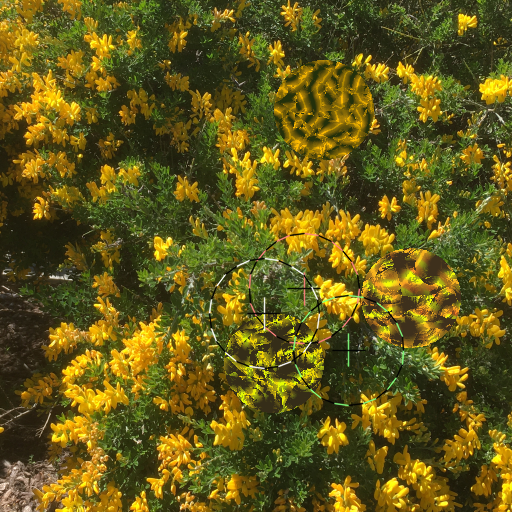
\includegraphics[scale=0.24]{20220930_step_6093}
    \hfill
    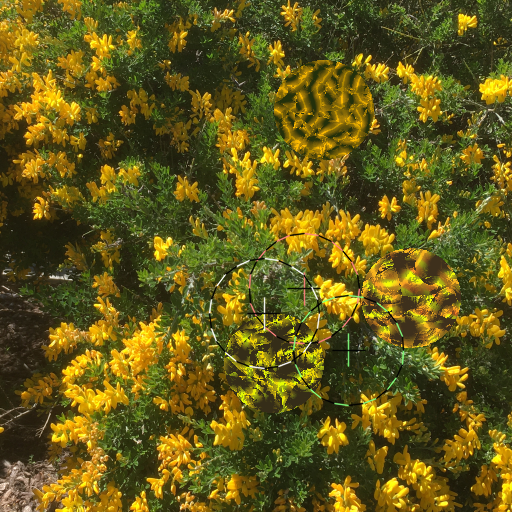
\includegraphics[scale=0.24]{20220930_step_6093}
    \hfill
    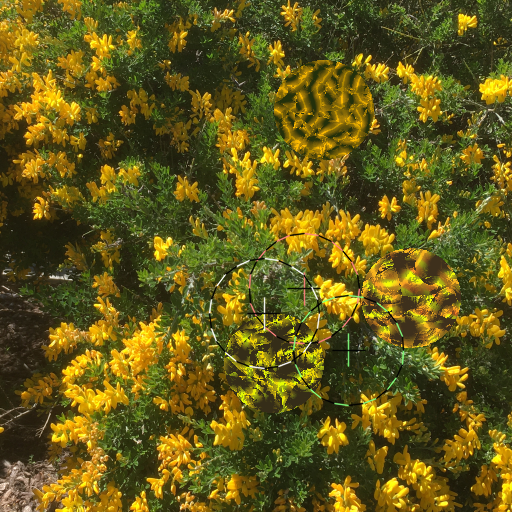
\includegraphics[scale=0.24]{20220930_step_6093}
    \hfill
    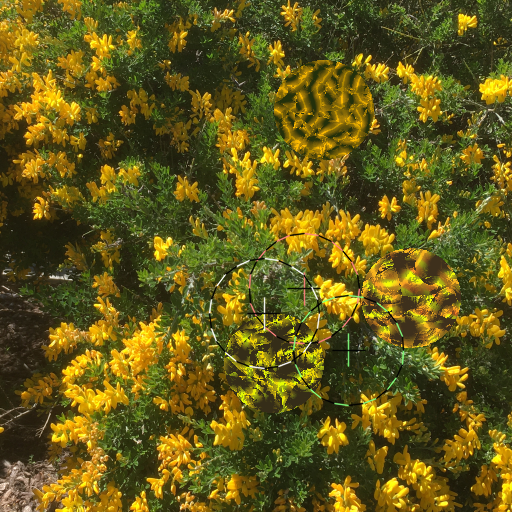
\includegraphics[scale=0.24]{20220930_step_6093}
    \caption{Teaser figure}
    \Description{This is the teaser figure for the article.}
    \label{fig:teaser}
\end{teaserfigure}

\maketitle

%% The actual document with your content starts here

\section{Introduction}
[... introduction ... following the approach of \citet{Reynolds2011} a population of prey, each with a synthetic camouflage texture, are evolved against negative selection by a predator which prefers the most conspicuous prey against a given background. ...]

\section{Related work}
[... xxx ...]

[... TexSyn is based on the “strongly typed” variant of Genetic Programming known as STGP \cite{montana_strongly_1995}, one of several grammar-based GP varients \cite{Mckay_2010}. ...]

%% Acknowledgements
\begin{acks}
Acknowledgements
\end{acks}

%% Bibliography.
%% Uncomment the bibliography line and link to an actual bib file
\bibliographystyle{ACM-Reference-Format}
% \bibliography{bibliography.bib}
\bibliography{coc.bib}


%% Appendix
\appendix

\section{Additional Section}

Text

\end{document}
